%\VignetteEngine{knitr::knitr}
%\VignetteDepends{ggplot2}
%\VignetteDepends{plyr}
%\VignetteDepends{dplyr}
%\VignetteDepends{reshape2}
%\VignetteIndexEntry{Basic ODE model fitting}
\documentclass{article}\usepackage[]{graphicx}\usepackage[]{color}
%% maxwidth is the original width if it is less than linewidth
%% otherwise use linewidth (to make sure the graphics do not exceed the margin)
\makeatletter
\def\maxwidth{ %
  \ifdim\Gin@nat@width>\linewidth
    \linewidth
  \else
    \Gin@nat@width
  \fi
}
\makeatother

\definecolor{fgcolor}{rgb}{0.345, 0.345, 0.345}
\newcommand{\hlnum}[1]{\textcolor[rgb]{0.686,0.059,0.569}{#1}}%
\newcommand{\hlstr}[1]{\textcolor[rgb]{0.192,0.494,0.8}{#1}}%
\newcommand{\hlcom}[1]{\textcolor[rgb]{0.678,0.584,0.686}{\textit{#1}}}%
\newcommand{\hlopt}[1]{\textcolor[rgb]{0,0,0}{#1}}%
\newcommand{\hlstd}[1]{\textcolor[rgb]{0.345,0.345,0.345}{#1}}%
\newcommand{\hlkwa}[1]{\textcolor[rgb]{0.161,0.373,0.58}{\textbf{#1}}}%
\newcommand{\hlkwb}[1]{\textcolor[rgb]{0.69,0.353,0.396}{#1}}%
\newcommand{\hlkwc}[1]{\textcolor[rgb]{0.333,0.667,0.333}{#1}}%
\newcommand{\hlkwd}[1]{\textcolor[rgb]{0.737,0.353,0.396}{\textbf{#1}}}%
\let\hlipl\hlkwb

\usepackage{framed}
\makeatletter
\newenvironment{kframe}{%
 \def\at@end@of@kframe{}%
 \ifinner\ifhmode%
  \def\at@end@of@kframe{\end{minipage}}%
  \begin{minipage}{\columnwidth}%
 \fi\fi%
 \def\FrameCommand##1{\hskip\@totalleftmargin \hskip-\fboxsep
 \colorbox{shadecolor}{##1}\hskip-\fboxsep
     % There is no \\@totalrightmargin, so:
     \hskip-\linewidth \hskip-\@totalleftmargin \hskip\columnwidth}%
 \MakeFramed {\advance\hsize-\width
   \@totalleftmargin\z@ \linewidth\hsize
   \@setminipage}}%
 {\par\unskip\endMakeFramed%
 \at@end@of@kframe}
\makeatother

\definecolor{shadecolor}{rgb}{.97, .97, .97}
\definecolor{messagecolor}{rgb}{0, 0, 0}
\definecolor{warningcolor}{rgb}{1, 0, 1}
\definecolor{errorcolor}{rgb}{1, 0, 0}
\newenvironment{knitrout}{}{} % an empty environment to be redefined in TeX

\usepackage{alltt}
\title{Basic ODE fitting}
\usepackage{amsmath}
\usepackage{natbib}
\usepackage{hyperref}
\newcommand{\rzero}{{\cal R}_0}
\newcommand{\code}[1]{{\tt #1}}
\bibliographystyle{chicago}
\date{\today}
\IfFileExists{upquote.sty}{\usepackage{upquote}}{}
\begin{document}
\maketitle



\section{Preliminaries}

Load packages:

\begin{knitrout}
\definecolor{shadecolor}{rgb}{0.969, 0.969, 0.969}\color{fgcolor}\begin{kframe}
\begin{alltt}
\hlkwd{library}\hlstd{(fitode)}
\hlkwd{library}\hlstd{(dplyr)}
\hlkwd{library}\hlstd{(ggplot2);} \hlkwd{theme_set}\hlstd{(}\hlkwd{theme_bw}\hlstd{())}
\hlkwd{library}\hlstd{(rbenchmark)}
\end{alltt}
\end{kframe}
\end{knitrout}

\section{SIR model}

Let's start with a simple case. This is how you define a model in fitode:

\begin{knitrout}
\definecolor{shadecolor}{rgb}{0.969, 0.969, 0.969}\color{fgcolor}\begin{kframe}
\begin{alltt}
\hlstd{sir} \hlkwb{<-} \hlkwd{new}\hlstd{(}\hlstr{"model.ode"}\hlstd{,}
    \hlstr{"sir model"}\hlstd{,}
    \hlkwc{model}\hlstd{=}\hlkwd{list}\hlstd{(}
        \hlstd{S} \hlopt{~ -}\hlstd{beta}\hlopt{*}\hlstd{S}\hlopt{*}\hlstd{I}\hlopt{/}\hlstd{N,}
        \hlstd{I} \hlopt{~} \hlstd{beta}\hlopt{*}\hlstd{S}\hlopt{*}\hlstd{I}\hlopt{/}\hlstd{N} \hlopt{-} \hlstd{gamma}\hlopt{*}\hlstd{I}
    \hlstd{),}
    \hlkwc{initial}\hlstd{=}\hlkwd{list}\hlstd{(}
        \hlstd{S} \hlopt{~} \hlstd{N}\hlopt{*}\hlstd{(}\hlnum{1}\hlopt{-}\hlstd{i0),}
        \hlstd{I} \hlopt{~} \hlstd{N}\hlopt{*}\hlstd{i0}
    \hlstd{),}
    \hlkwc{par}\hlstd{=}\hlkwd{c}\hlstd{(}\hlstr{"beta"}\hlstd{,} \hlstr{"gamma"}\hlstd{,} \hlstr{"N"}\hlstd{,} \hlstr{"i0"}\hlstd{)}

\hlstd{)}
\end{alltt}
\end{kframe}
\end{knitrout}

To solve this ode, one can use `ode.solve` function.

\begin{knitrout}
\definecolor{shadecolor}{rgb}{0.969, 0.969, 0.969}\color{fgcolor}\begin{kframe}
\begin{alltt}
\hlstd{time} \hlkwb{<-} \hlkwd{c}\hlstd{(}\hlnum{1}\hlopt{:}\hlnum{10}\hlstd{)}
\hlstd{par} \hlkwb{<-} \hlkwd{c}\hlstd{(}\hlkwc{beta}\hlstd{=}\hlnum{2}\hlstd{,} \hlkwc{gamma}\hlstd{=}\hlnum{1}\hlstd{,} \hlkwc{N}\hlstd{=}\hlnum{1000}\hlstd{,} \hlkwc{i0}\hlstd{=}\hlnum{1}\hlopt{/}\hlnum{1000}\hlstd{)}
\hlstd{ss} \hlkwb{<-} \hlkwd{ode.solve}\hlstd{(sir, time, par)}
\hlkwd{plot}\hlstd{(ss}\hlopt{@}\hlkwc{solution}\hlstd{)}
\end{alltt}
\end{kframe}
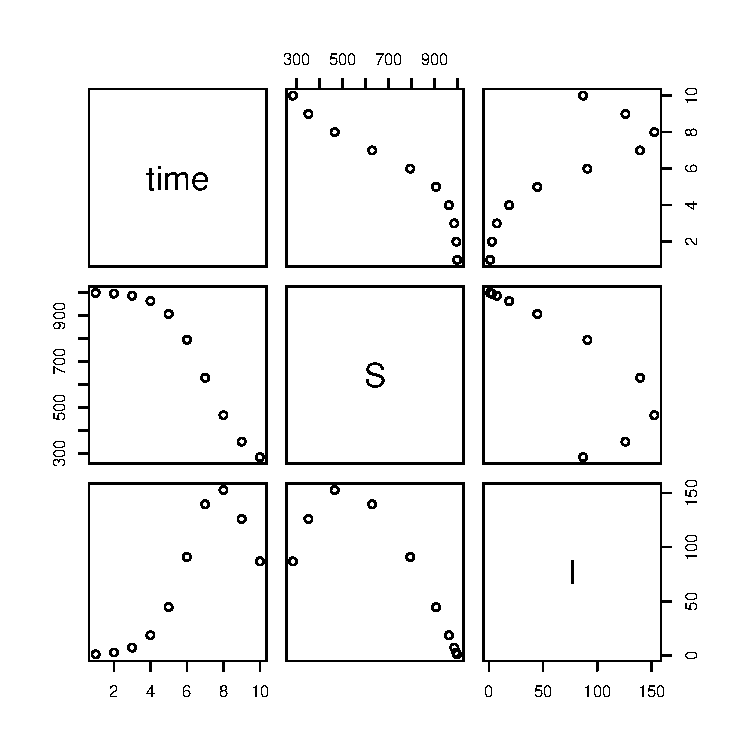
\includegraphics[width=\maxwidth]{figure/sir_model_solve-1} 

\end{knitrout}

\subsection{Fitting a model to Harbin Plague data}

Here's a simple fitting (note that all log likelihood parameters start with prefix `ll.`):

\begin{knitrout}
\definecolor{shadecolor}{rgb}{0.969, 0.969, 0.969}\color{fgcolor}\begin{kframe}
\begin{alltt}
\hlstd{harbin} \hlkwb{<-} \hlstd{fitsir}\hlopt{::}\hlstd{harbin}

\hlstd{start} \hlkwb{<-} \hlkwd{c}\hlstd{(}\hlkwc{beta}\hlstd{=}\hlnum{2}\hlstd{,} \hlkwc{gamma}\hlstd{=}\hlnum{1}\hlstd{,} \hlkwc{N}\hlstd{=}\hlnum{1e5}\hlstd{,} \hlkwc{i0}\hlstd{=}\hlnum{1e-4}\hlstd{,} \hlkwc{ll.sigma}\hlstd{=}\hlnum{5}\hlstd{)}

\hlstd{ff} \hlkwb{<-} \hlkwd{fitode}\hlstd{(Deaths}\hlopt{|}\hlstd{week}\hlopt{~}\hlstd{gamma}\hlopt{*}\hlstd{I,}
    \hlkwc{start}\hlstd{=start,}
    \hlkwc{model}\hlstd{=sir,}
    \hlkwc{loglik}\hlstd{=}\hlkwd{select_model}\hlstd{(}\hlstr{"gaussian"}\hlstd{),}
    \hlkwc{data}\hlstd{=harbin}
\hlstd{)}


\hlkwd{print}\hlstd{(ff)}
\end{alltt}
\begin{verbatim}
## Model: sir model 
## Formula: Deaths | week ~ gamma * I 
## 
## Coefficients:
##          beta         gamma             N            i0      ll.sigma 
## -1.018694e+00  1.158019e-02  1.000000e+05  4.841317e-03  1.190017e+02 
## 
## Log-Likelihood:-105.36 
## 
## link: log.ll.sigma
\end{verbatim}
\end{kframe}
\end{knitrout}

With this starting parameter, `fitode` fails to find mle. We can improve the fit by using link functions:

\begin{knitrout}
\definecolor{shadecolor}{rgb}{0.969, 0.969, 0.969}\color{fgcolor}\begin{kframe}
\begin{alltt}
\hlstd{ff2} \hlkwb{<-} \hlkwd{fitode}\hlstd{(Deaths}\hlopt{|}\hlstd{week}\hlopt{~}\hlstd{gamma}\hlopt{*}\hlstd{I,}
    \hlkwc{start}\hlstd{=start,}
    \hlkwc{model}\hlstd{=sir,}
    \hlkwc{loglik}\hlstd{=}\hlkwd{select_model}\hlstd{(}\hlstr{"gaussian"}\hlstd{),}
    \hlkwc{data}\hlstd{=harbin,}
    \hlkwc{link}\hlstd{=}\hlkwd{list}\hlstd{(}
        \hlkwc{beta}\hlstd{=}\hlstr{"log"}\hlstd{,}
        \hlkwc{gamma}\hlstd{=}\hlstr{"log"}\hlstd{,}
        \hlkwc{N}\hlstd{=}\hlstr{"log"}\hlstd{,}
        \hlkwc{i0}\hlstd{=}\hlstr{"logit"}
    \hlstd{)}
\hlstd{)}
\hlkwd{print}\hlstd{(ff2)}
\end{alltt}
\begin{verbatim}
## Model: sir model 
## Formula: Deaths | week ~ gamma * I 
## 
## Coefficients:
##         beta        gamma            N           i0     ll.sigma 
## 1.623168e+00 7.704775e-01 1.815253e+03 4.892969e-04 1.334958e+01 
## 
## Log-Likelihood:-68.18 
## 
## link: log.beta log.gamma log.N logit.i0 log.ll.sigma
\end{verbatim}
\end{kframe}
\end{knitrout}

We can look at the predicted trajectory:

\begin{knitrout}
\definecolor{shadecolor}{rgb}{0.969, 0.969, 0.969}\color{fgcolor}\begin{kframe}
\begin{alltt}
\hlkwd{plot}\hlstd{(ff2,} \hlkwc{level}\hlstd{=}\hlnum{0.95}\hlstd{)}
\end{alltt}
\end{kframe}
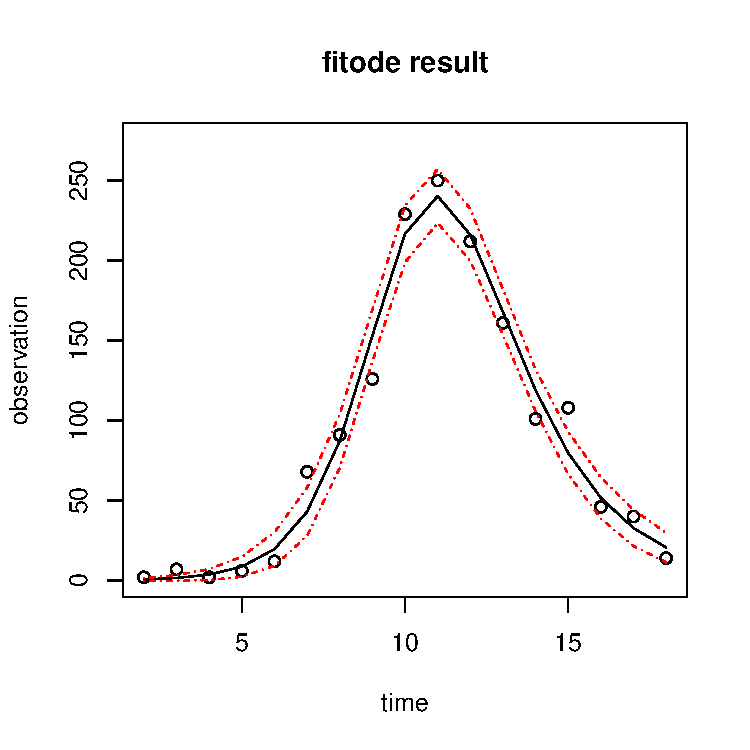
\includegraphics[width=\maxwidth]{figure/plot-1} 

\end{knitrout}

This looks pretty good but we are not dealing with overdispersion properly.

\begin{knitrout}
\definecolor{shadecolor}{rgb}{0.969, 0.969, 0.969}\color{fgcolor}\begin{kframe}
\begin{alltt}
\hlstd{start2} \hlkwb{<-} \hlkwd{c}\hlstd{(}\hlkwd{coef}\hlstd{(ff2)[}\hlnum{1}\hlopt{:}\hlnum{4}\hlstd{],} \hlkwc{ll.phi}\hlstd{=}\hlnum{2}\hlstd{)}

\hlstd{ff3} \hlkwb{<-} \hlkwd{fitode}\hlstd{(Deaths}\hlopt{|}\hlstd{week}\hlopt{~}\hlstd{gamma}\hlopt{*}\hlstd{I,}
    \hlkwc{start}\hlstd{=start2,}
    \hlkwc{model}\hlstd{=sir,}
    \hlkwc{loglik}\hlstd{=}\hlkwd{select_model}\hlstd{(}\hlstr{"nbinom1"}\hlstd{),}
    \hlkwc{data}\hlstd{=harbin,}
    \hlkwc{link}\hlstd{=}\hlkwd{list}\hlstd{(}
        \hlkwc{beta}\hlstd{=}\hlstr{"log"}\hlstd{,}
        \hlkwc{gamma}\hlstd{=}\hlstr{"log"}\hlstd{,}
        \hlkwc{N}\hlstd{=}\hlstr{"log"}\hlstd{,}
        \hlkwc{i0}\hlstd{=}\hlstr{"logit"}
    \hlstd{)}
\hlstd{)}

\hlkwd{print}\hlstd{(ff3)}
\end{alltt}
\begin{verbatim}
## Model: sir model 
## Formula: Deaths | week ~ gamma * I 
## 
## Coefficients:
##         beta        gamma            N           i0       ll.phi 
## 1.714493e+00 9.226696e-01 1.998729e+03 5.503243e-04 1.795928e+00 
## 
## Log-Likelihood:-64.59 
## 
## link: log.beta log.gamma log.N logit.i0 log.ll.phi
\end{verbatim}
\end{kframe}
\end{knitrout}

Compare the plots...

\begin{knitrout}
\definecolor{shadecolor}{rgb}{0.969, 0.969, 0.969}\color{fgcolor}\begin{kframe}
\begin{alltt}
\hlkwd{plot}\hlstd{(ff3,} \hlkwc{level}\hlstd{=}\hlnum{0.95}\hlstd{,} \hlkwc{col.traj}\hlstd{=}\hlnum{1}\hlstd{,} \hlkwc{col.conf}\hlstd{=}\hlnum{1}\hlstd{)}
\hlkwd{plot}\hlstd{(ff2,} \hlkwc{level}\hlstd{=}\hlnum{0.95}\hlstd{,} \hlkwc{col.traj}\hlstd{=}\hlnum{2}\hlstd{,} \hlkwc{col.conf}\hlstd{=}\hlnum{2}\hlstd{,} \hlkwc{add}\hlstd{=}\hlnum{TRUE}\hlstd{)}
\hlkwd{legend}\hlstd{(}\hlnum{2}\hlstd{,} \hlnum{250}\hlstd{,} \hlkwc{legend}\hlstd{=}\hlkwd{c}\hlstd{(}\hlstr{"nbinom1"}\hlstd{,} \hlstr{"gaussian"}\hlstd{),} \hlkwc{col}\hlstd{=}\hlkwd{c}\hlstd{(}\hlnum{1}\hlstd{,}\hlnum{2}\hlstd{),} \hlkwc{lty}\hlstd{=}\hlnum{1}\hlstd{)}
\end{alltt}
\end{kframe}
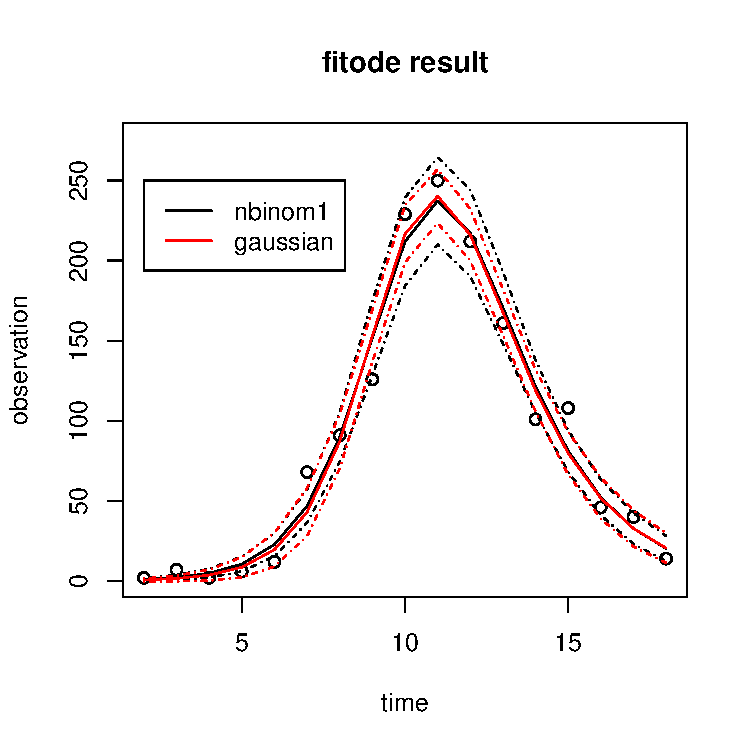
\includegraphics[width=\maxwidth]{figure/plot2-1} 

\end{knitrout}



\end{document}
